\problemname{Message}
\noindent
In the city where Paula lives, there is a large square. 
The square can be represented as a grid with $N$ rows and $M$ columns. 
Some of the grid cells contain engraved letters.

According to a legend, these letters form a message if one walks on the cells 
in a specific order. To make it correct, one must start in the upper-left 
corner and end in the lower-right corner, by only moving right and downward. 
If one manages to visit all cells with engraved letters in this way, 
the secret message will be revealed.

Paula has decided to crack the mystery once and for all and find the secret message.

Write a program that finds the message given the grid.

\section*{Input}
The first line contains two integers $N$ and $M$ ($1 \leq N, M \leq 6$), 
the number of rows and columns in the grid.

The following $N$ lines contain a string of length $M$ each. 
These strings represent the rows in the grid and contain lowercase 
letters \texttt{a}-\texttt{z} and dots ``.''. The dots represent empty cells.

It is guaranteed that it is possible to visit all cells with engraved letters 
by starting in the upper-left corner and moving right and downward to the lower-right corner.

\section*{Output}
Print a string, the secret message.

\section*{Points}
Your solution will be tested on several test case groups.
To get the points for a group, it must pass all the test cases in the group.

\noindent
\begin{tabular}{| l | l | p{12cm} |}
  \hline
  \textbf{Group} & \textbf{Point value} & \textbf{Constraints} \\ \hline
  $1$    & $20$       & $N = 1$ \\ \hline
  $2$    & $40$       & The number of letters is $N+M-1$. \\ \hline
  $3$    & $40$       & No additional constraints. \\ \hline
\end{tabular}

\section*{Explanation of sample 1}

\begin{figure}[h]
    \centering
    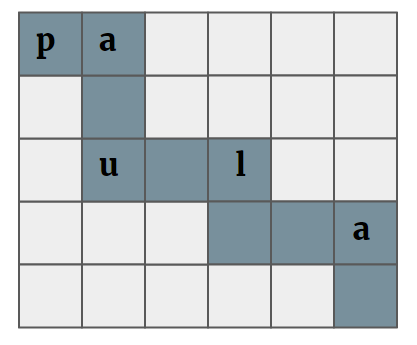
\includegraphics[width=0.3\textwidth]{sample.PNG}
      \\The image shows the solution to sample case 1. The dark cells 
      represent a possible way to go from the upper-left corner to the 
      lower-right corner, visiting all letters.
    
  \end{figure}
